\documentclass[a4paper,10pt, twocolumn]{article}
\usepackage{graphicx}
\usepackage[english]{babel}
\usepackage{geometry}           
\geometry{letterpaper}                   
\usepackage{graphicx}
\usepackage{amsmath}
\usepackage{amssymb}
\usepackage{graphicx,wrapfig,lipsum}
\usepackage{listings}
\usepackage{subfigure}
\usepackage{wrapfig}
\usepackage{url}
\usepackage[section]{placeins}
\usepackage{fontspec,xltxtra,xunicode}
\usepackage{todonotes}

\title{Three-Dimensional Vizualization and Animation\\Technical Report - Assignment III.}
\author{
  Marfeychuk, Mykhaylo\\
  \texttt{ist194039}
  \and
  Skalický, Matyáš\\
  \texttt{ist194904}
}

\date{} % 31.10.2019

\begin{document}
\maketitle

%\begin{figure}[!htb]
%	\centering
% 	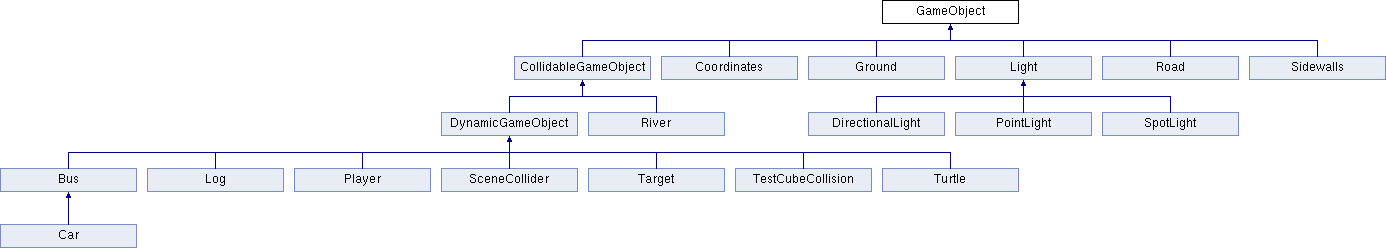
\includegraphics[width=\linewidth]{images/image1.png}
%  	\caption{Objects which inherit from the GameObject class.}
%\end{figure}

\section*{Introduction}
The following document describes the work on the task 3, the development of the frogger game in the ThreeJS framework.

\section{Cameras and stereo effect}
The application contains several cameras. The player can switch the camera using the keys 1 to 5. All of the cameras also show information about the game except for the stereo mode, for which we do not show any information on the screen to make the screen less cluttered.

\begin{figure}[!htb]
	\centering
 	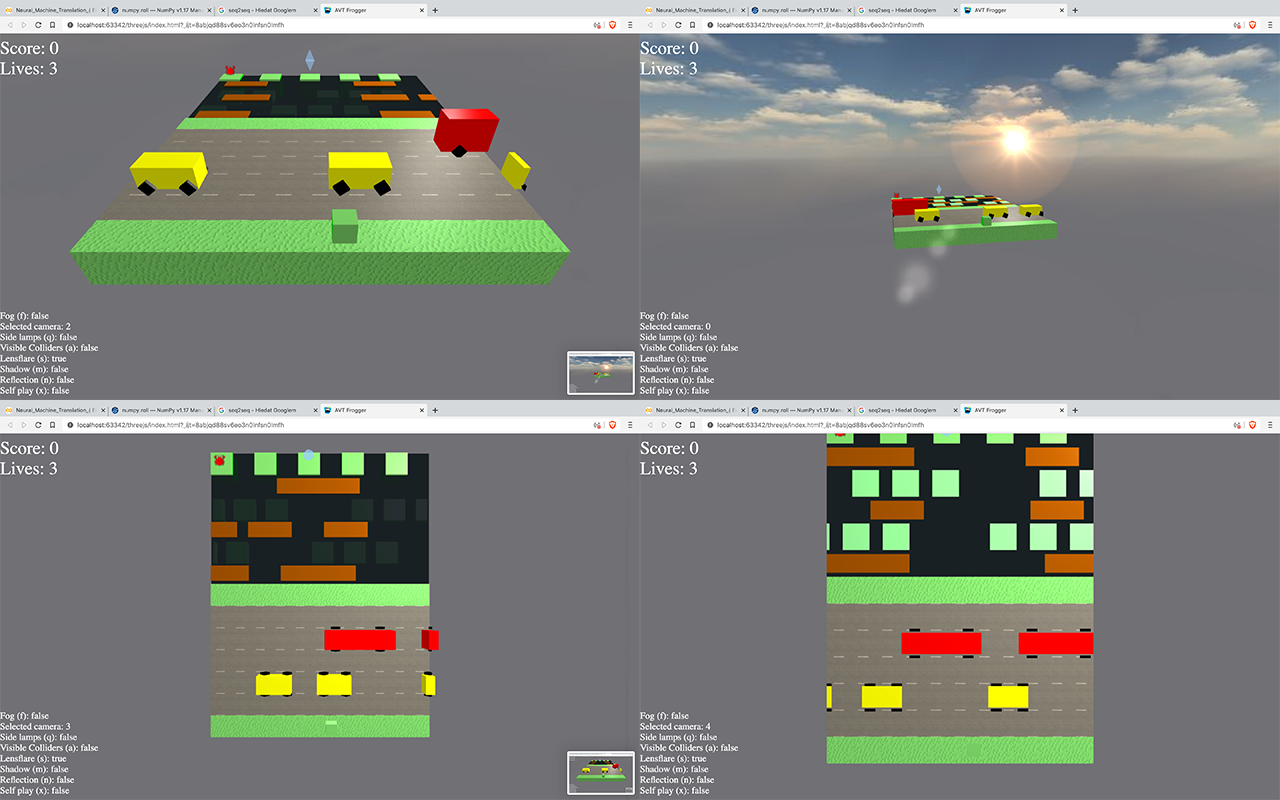
\includegraphics[width=\linewidth]{images/cam_merged.png}
  	\caption{From top left: perspective following camera, rotating perspective camera, top perspective camera and top orthogonal camera.}
	\label{cameras}
\end{figure}

The stereo viewing was implemented based on the module provided on the ThreeJS demo accessible at \url{https://threejs.org/examples/webgl_effects_stereo.html}. 

\begin{figure}[!htb]
	\centering
 	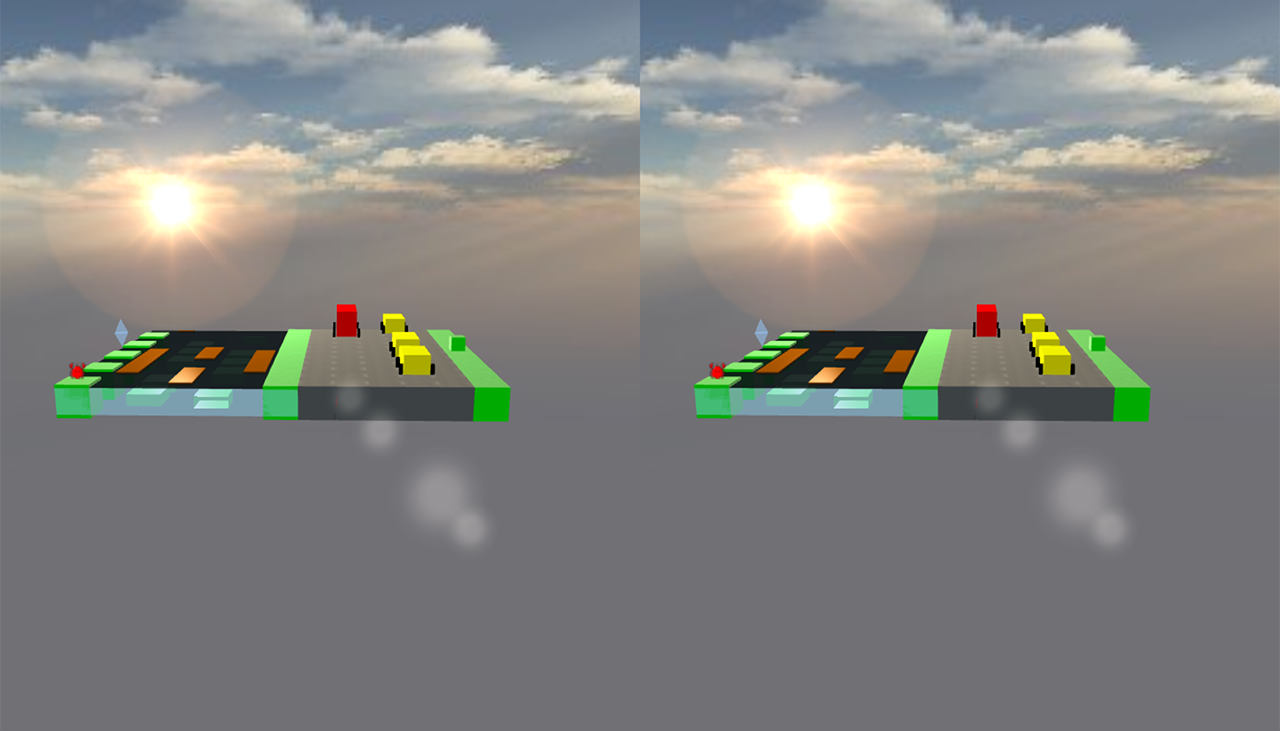
\includegraphics[width=\linewidth]{images/cam_stereo.png}
  	\caption{Stereo perspective rotating camera.}
	\label{stereocam}
\end{figure}

\section{Object movement and collision detection}
Each frame, we first check the collisions, update the game objects positions and then draw them to the screen. 

Collision detection is done by checking the collision of the player and all of the collidable game objects each frame. ThreeJS makes this very easy as we can easily precalculate the bounding box for a given geometry and then easily check for collisions between them. 


\section{Lights}
The directional light can be seen on the Figure \ref{cameras}. The 8 point lights in the scene can be toggled with the usage of \emph{q} key. We used the built-in ThreeJS light classes.

\begin{figure}[!htb]
	\centering
 	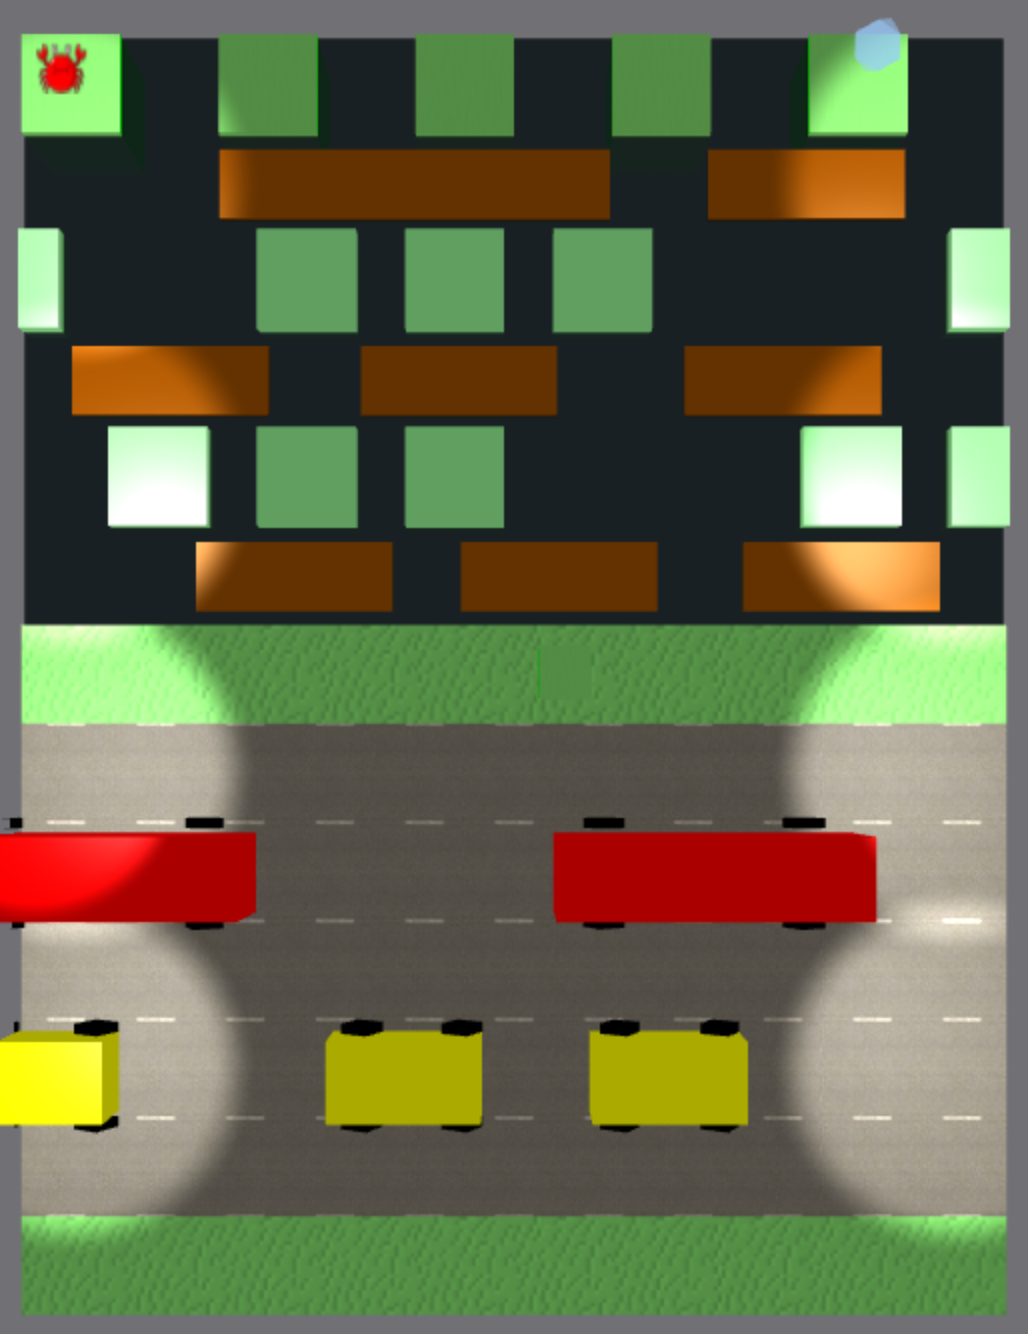
\includegraphics[width=0.7\linewidth]{images/pointlights.png}
  	\caption{Pointlights activated.}
	\label{pointlights}
\end{figure}

\section{Scoring system}
Scene contains the current score on the top of the screen as shown on the Figure \ref{score}. The score is increased when the player reaches the target crystal on the other side of the river and the game also speeds up to get harder.

\begin{figure}[!htb]
	\centering
 	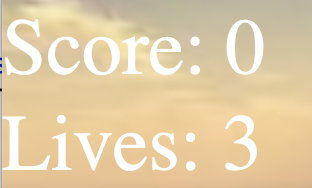
\includegraphics[width=0.5\linewidth]{images/score.png}
  	\caption{Scoring.}
	\label{score}
\end{figure}


\section{Fog}
Creating fog in ThreeJS is done simply by using the \lstinline{THREE.Fog()} class. User can toggle the fog on and off using the f key. The result is shown on the Figure \ref{fog}.

\begin{figure}[!htb]
	\centering
	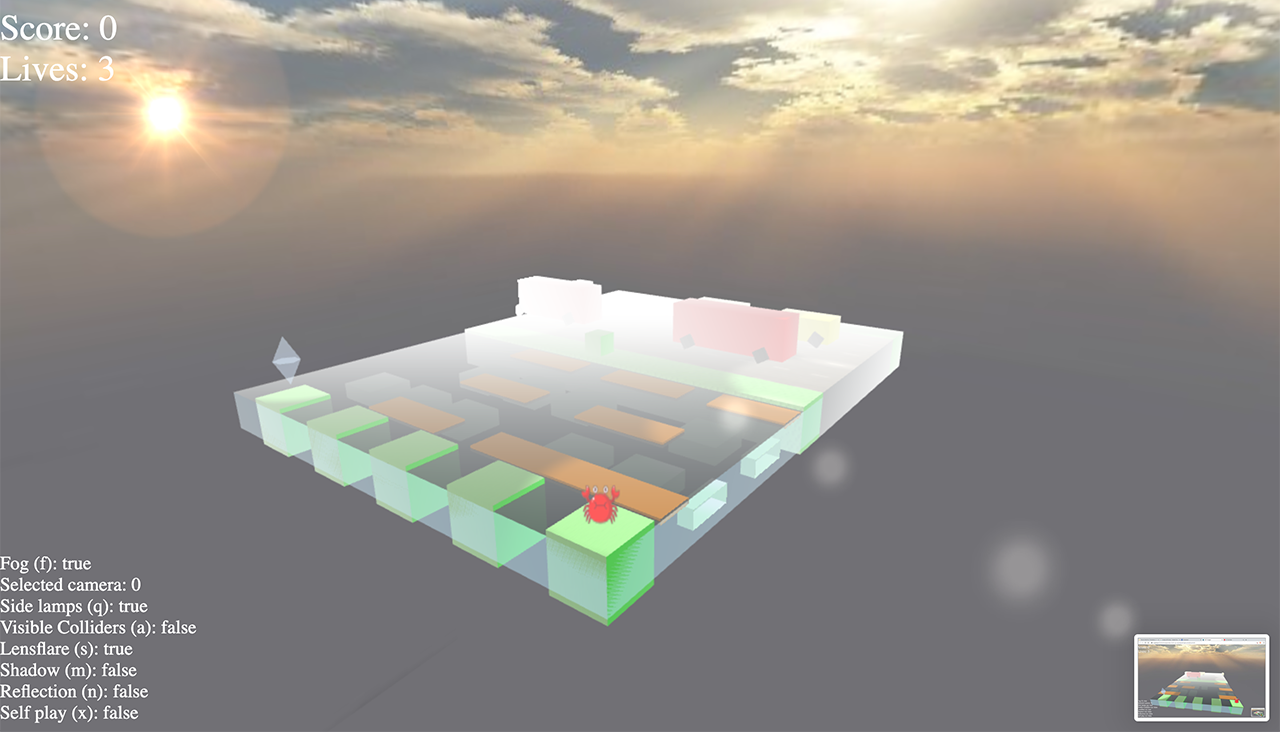
\includegraphics[width=\linewidth]{images/fog.png}
  	\caption{Fog.}
	\label{fog}
\end{figure}

\section{Planar reflections and shadows}
The planar reflection is implemented using a cube camera positioned on the other side of the plane which is then projected to the surface of the water. This effect, where the skybox is projected can be seen in the Figure \ref{reflection}.

\begin{figure}[!htb]
	\centering
 	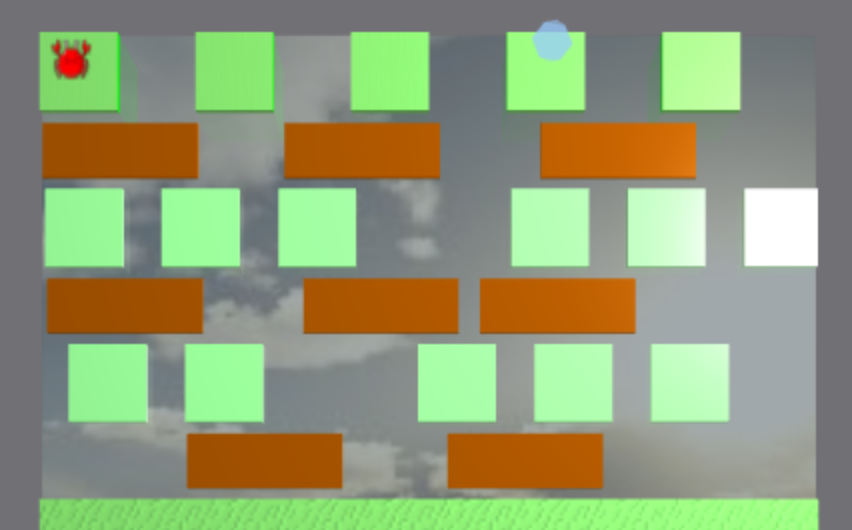
\includegraphics[width=\linewidth]{images/reflection.png}
  	\caption{Reflection.}
	\label{reflection}
\end{figure}

The shadows are created by using the native  Three.js framework methods, which already does all the necessary to render the shadows. The framework first renders the models onto a plane, and then renders the real object on top. The shadows can be seen in Figure \ref{shadow}.

\begin{figure}[!htb]
	\centering
	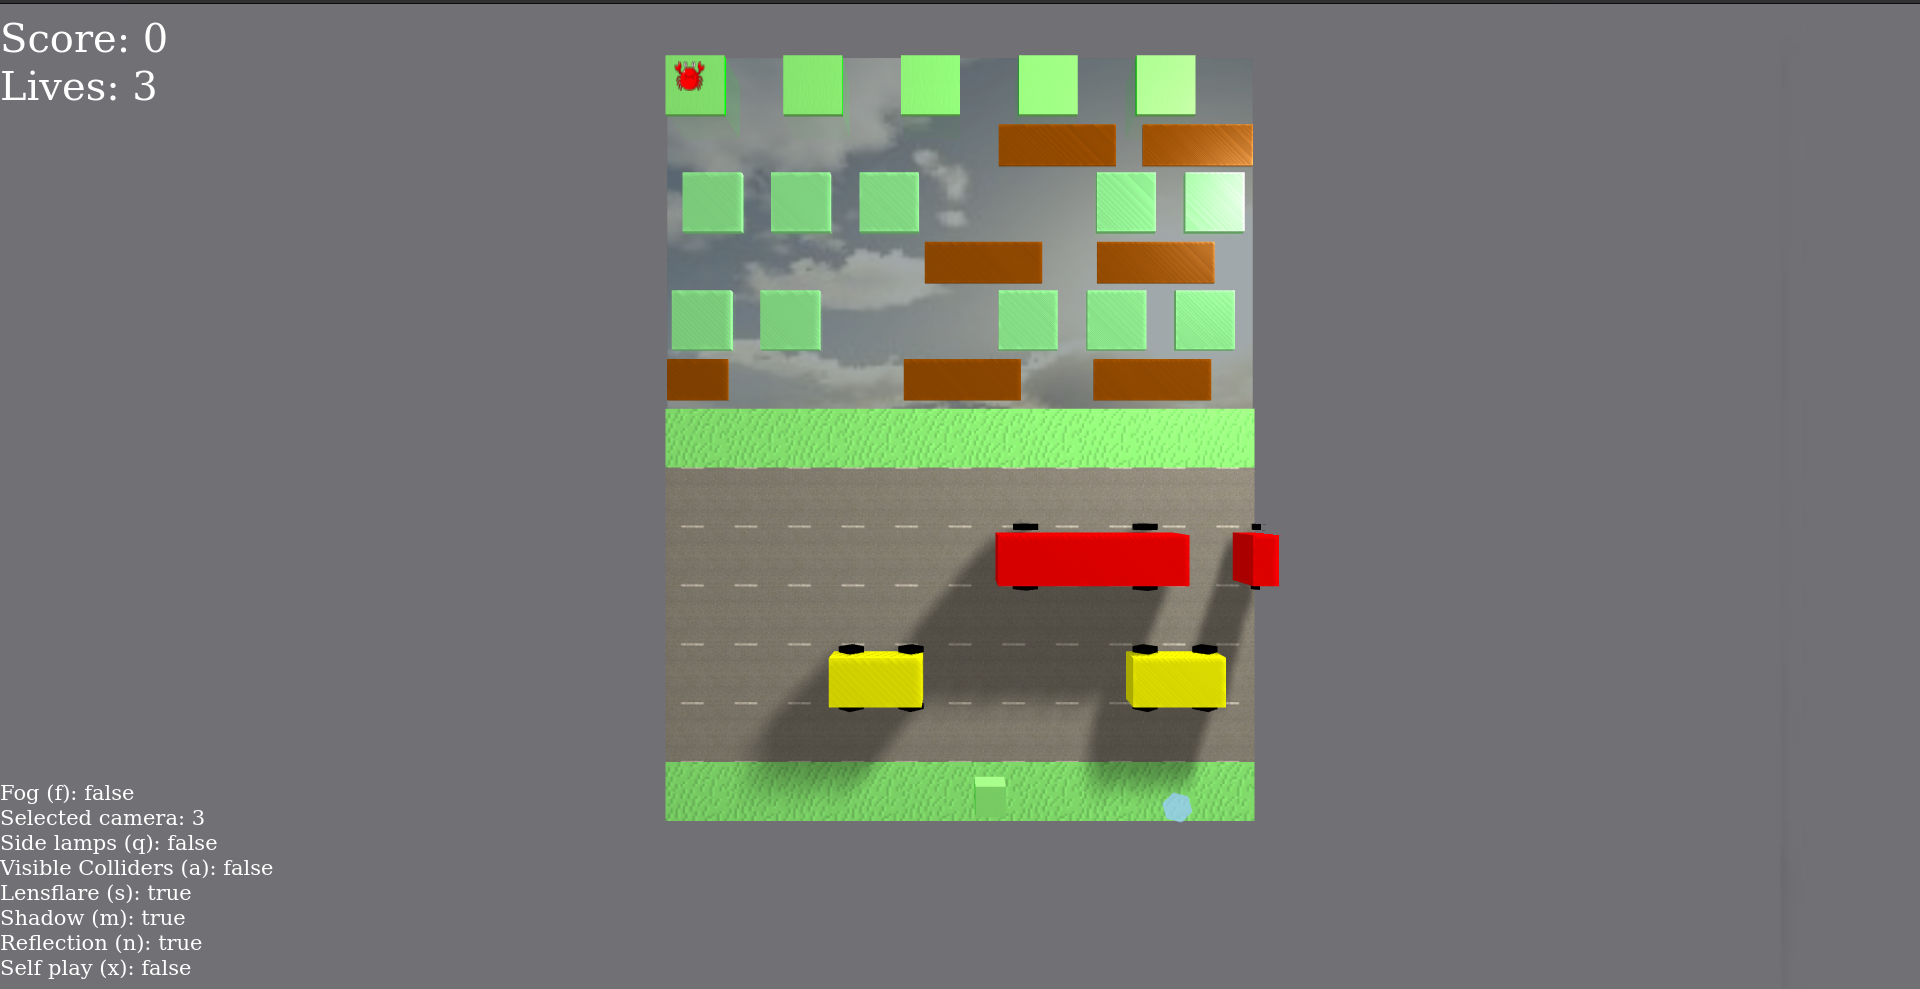
\includegraphics[width=\linewidth]{images/shadows.png}
  	\caption{Shadow.}
	\label{shadow}
\end{figure}

\section{Billboard}
We used a little crab to demonstrate the usage of billboards in our game. This can be seen for example on the Figure \ref{fog}.

\section{Lens flare}
For our demo, we have utilized the ThreeJS Lensflare class, which makes the lens flares very easy. the lens flare is located at the ``sun'' in the sky and can be seen on the Figure \ref{lensflare}.

\begin{figure}[!htb]
	\centering
	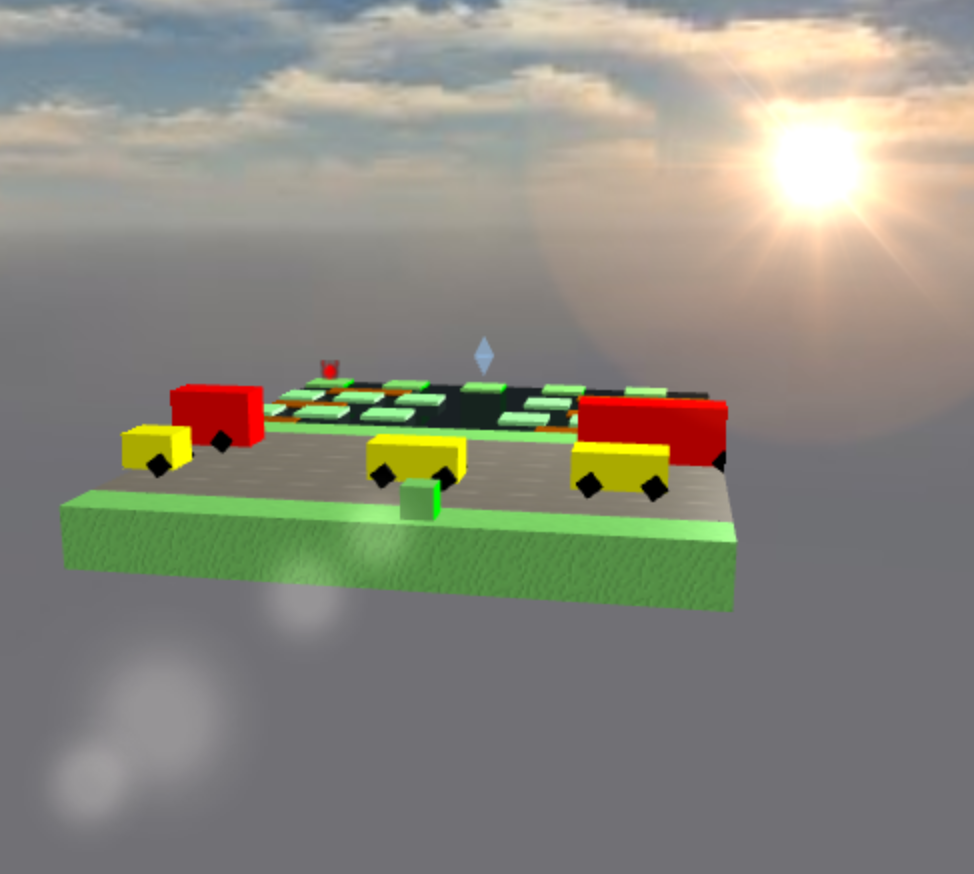
\includegraphics[width=\linewidth]{images/lensflare.png}
	\caption{Lens flare.}
	\label{lensflare}
\end{figure}

\section{Texturing and skybox}
ThreeJS allows the developers to write custom shaders for a material. The skybox is done using a large cube textured with a custom GLSL shader cube map. The skybox can be seen on the Figure \ref{fog}.

We gave textured the ground with a grass texture as well as the road with the road stripes texture.

\section{Other features}
We have used the clipping mechanism to remove the objects which come into the scene and also go away. 

We have also implemented the autoplay. User can activate the auto-play feature to test the game when using the VR glasses. This is done by pressing the \emph{x} key.

\section*{Conclusion}
We have implemented most of the required functionality for the third task of our project. Sadly, due to time contains and also one of our group member missing, we have not implemented the bump-mapping and a particle system. The mobile gyroscope controls were developed, however we ran into a technical problem  with hosting. Mobile browser is not able to access the gyro data over http and our hosting does not have the SSL set up. 

The testing was difficult as Matyáš's old phone did not run any of the WebGL content, and Mykhaylo's phone was too large to fit into the Google Glass headset. 

We have ported most of the functionality from the original C++ game into the modern ThreeJS environment. Development in ThreeJS is incomparably simpler than the low-level C. 

\end{document}  